\documentclass[class=report, crop=false, 12pt,a4paper, tikz, border=4mm]{standalone}
\usepackage{enumitem}
\usepackage{tikz}
\usepackage{float}
\usepackage[normalem]{ulem}
\usepackage{graphicx}
\usepackage{siunitx}
\usepackage{tikz}
\usetikzlibrary{positioning, fit, calc}   
\tikzset{block/.style={draw, thick, text width=3cm ,minimum height=1.3cm, align=center},   
line/.style={-latex}     
}   
\begin{document}
A measurement system has to be devised such that the relationship between the real value of a variable and the value actually measured is unambiguously known. For example, when placing a weight on a scale, we must know the relationship between the \textbf{true} weight and the \textbf{measured} weight. 
\begin{figure}
  \centering
  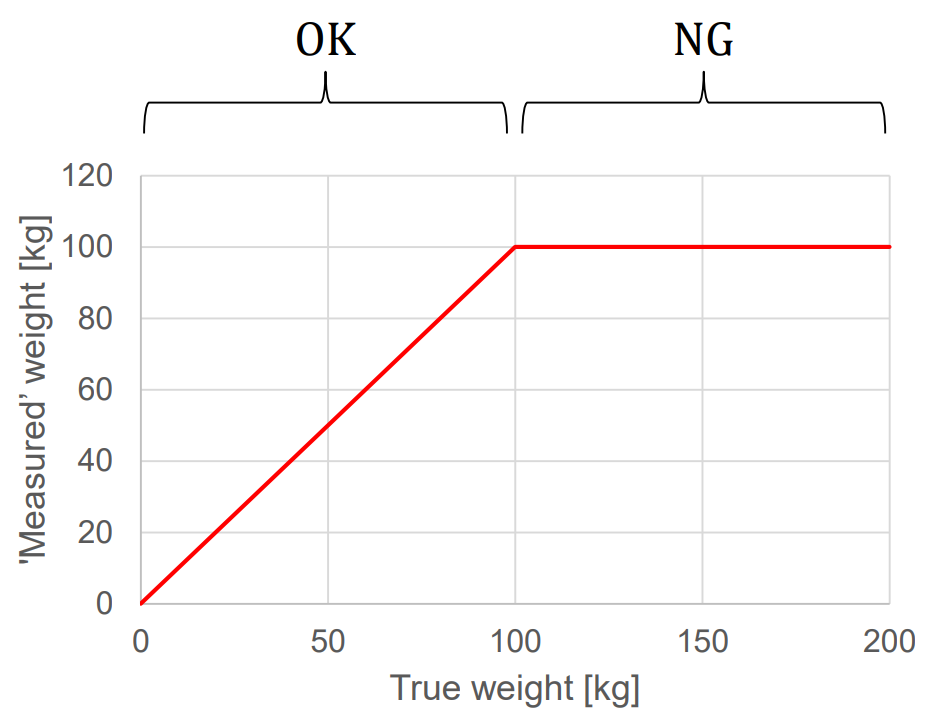
\includegraphics[width = 0.6\textwidth]{../img/rsbetweentrueandmeasured.png}
  \caption{The scales work well up to 100kg, however it may not be able to measure heavier weights effectively.}
\end{figure}
The measurement system must allow:
\begin{itemize}
  \item Easy interpretation of the measured data
  \item Provide high degree of confidence
\end{itemize}
\begin{figure}
  \centering
  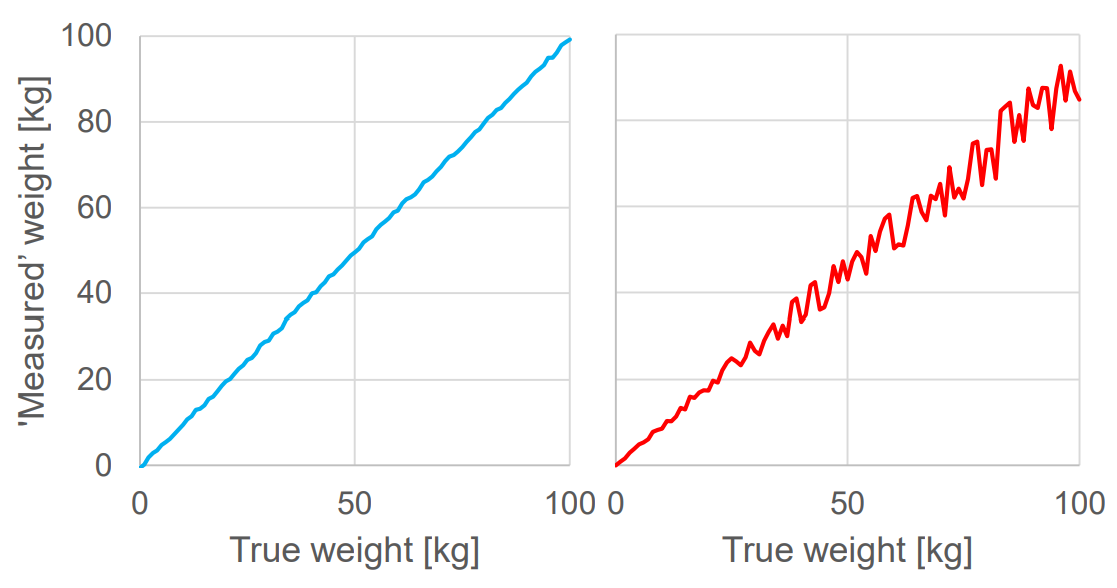
\includegraphics[width=0.6\textwidth]{../img/electricscalegraphs.png}
  \caption{On the red graph we can see the effect that noise has on our measurement - a source of an inaccuracy. This must be dealt with to have an effective measurement system.}
\end{figure}
\begin{figure}
  \centering
  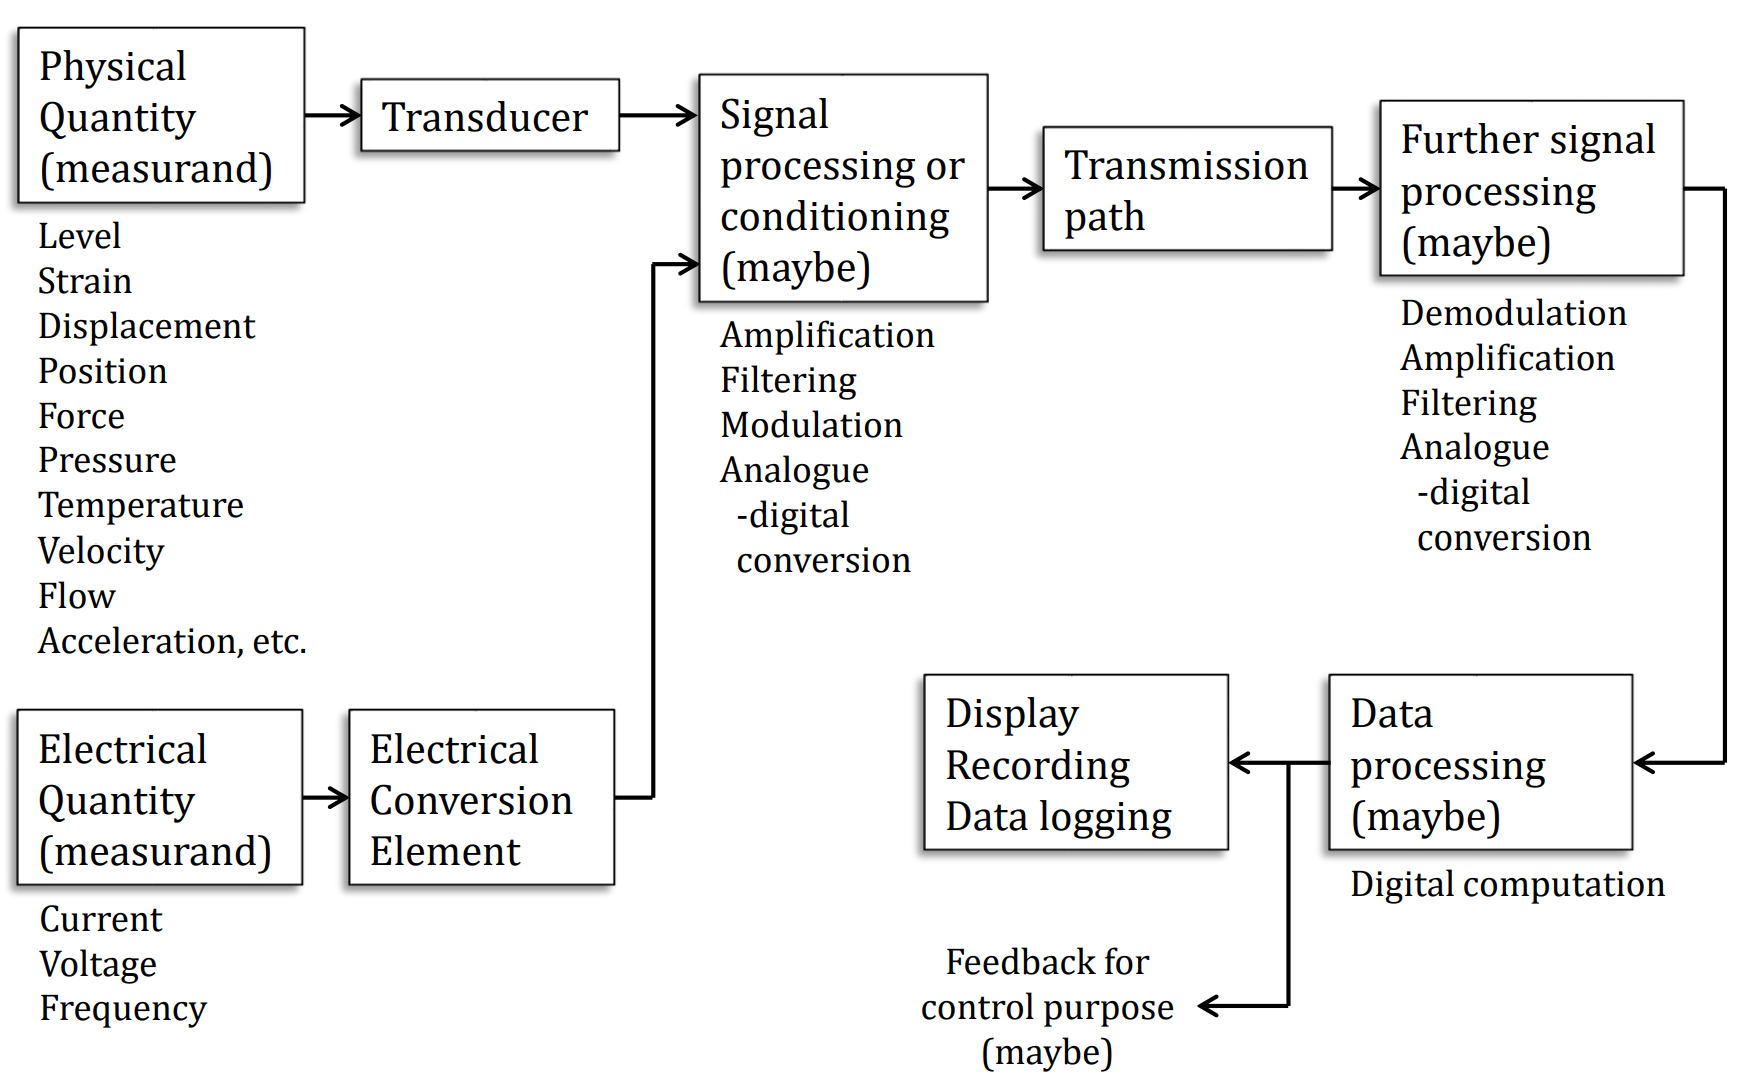
\includegraphics[width=0.8\textwidth]{../img/generalmeasurementsystem.png}
  \caption{Block diagram to show a general measurement system.}
\end{figure}

\begin{figure}
  \centering
  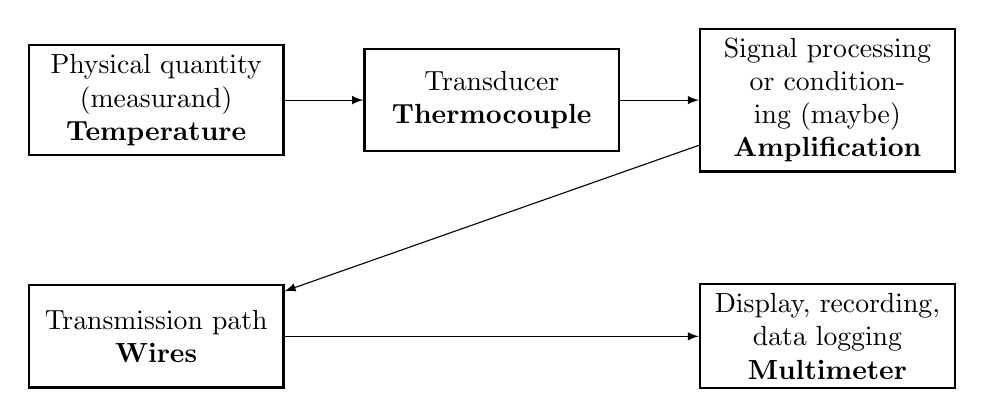
\begin{tikzpicture}
    \node[block] (a) {Physical quantity (measurand) \textbf{Temperature}};
    \node[block, right= of a] (b) {Transducer \textbf{Thermocouple}};
    \node[block, right= of b] (c) {Signal processing or conditioning (maybe) \textbf{Amplification}};
    \node[block] (d) at ([yshift = -3cm]$(a)!1.0!(a)$) {Transmission path \\ \textbf{Wires}};
    \node[block] (e) at ([yshift = -3cm]$(c)!1.0!(c)$) {Display, recording, data logging \textbf{Multimeter}};

    \draw[line] (a)-- (b);  
    \draw[line] (b)-- (c);  
    \draw[line] (c)-- (d);
    \draw[line] (d)-- (e);
  \end{tikzpicture}
  \caption{How the workflow of a measurement can be constructed.}
\end{figure}
\section{Transducers}
A transducer converts the sensed variable into a detectable signal form. Sometimes the device changes a mechanical quantity into a change in an  electrical quantity. For example, a strain gauge converts a change in strain in the specimen to a change in electrical resistance in the gauge. Another example is a thermometer which converts thermal expansion of the liquid (due to a rise in temperature) into a mechanical translation.
\section{Signal condition circuits}
This takes the transducer signal and can convert, compensate or manipulate it into a more usable electrical quantity. This may include filters, compensators, modulators, demodulators, integrators or differentiators. For example, a Wheatstone bridge used with the strain gauge converts the change in the electrical resistance of the gauge to a change in voltage.
\section{Amplifiers}
They are required in systems when the output from the transducer-signal conditions is small. Gains of 10 - 1000 are used to increase the levels of the signal, typically a millivolt or less, to what is compatible with the voltage-measuring devices used in the system. A negative-feedback amplifier circuit is an example of an amplifier.
\section{Output stage}
Generally, it is a voltage measurement device that is used to display the measurement in a form that can be read and interpreted. For example, digital voltmeters, self-balancing potentiometers, oscilloscopes, chart recorders and magnetic tape recorders.
\section{Feedback-control stage}
Used when the measurement system is employed in process control. The signal from the measurement system is compared with the command signal that reflects the required value of the quantity in the process. The process-controller forms the difference between these two and produces and error signal. The error signal is then used to automatically adjust the process. For example, the float system in a toilet (called a ballock) to control the water supply in the tank.
\section{Calibration}
How do we know whether one metre is one metre? We compare it with a reference, which is supposed to be reliable. This act of checking is called calibration. Our references are the measuring \textbf{standards}.
\section{Standards}
There are seven fundamental quantities of the International Measuring System.
\begin{itemize}
  \item Length \si{\m} - metre
  \item Time \si{\second} - second
  \item Mass \si{\kg} - kilogram
  \item Temperature \si{\kelvin} - kelvin
  \item Electric Current \si{\ampere} - ampere
  \item Luminous Intensity - \si{\candela} - candela
  \item Amount of Substance - \si{\mol} - mole
\end{itemize}
Units and standard for all other quantities are derived from these.

We can look at how the definition of the metre has changed over the past 2 centuries for some insight into the accuracy of our reference.
\begin{itemize}
  \item 1792 - a ten millionth of the quarter of a meridian ($0.5 - 0.1 \si{\milli\m}$ of uncertainty)
  \item 1889 - a platinum-iridium bar at melting point of ice ($0.2-0.1 \si{\micro\m}$ of uncertainty)
  \item 1983 - the length of the path travelled by light in vacuum during a time interval of $1/299792458$ of a second ($0.1 \si{\nano\m}$ of uncertainty)
\end{itemize}
Here are how the other fundamental quantities are defined.
\begin{itemize}
  \item Metre - Length of the path travelled by light in a vacuum in $1/299792458$ of a second
  \item Time - Duration of $9192631770$ periods of the radiation corresponding to the transition between the two hyperfine levels of the ground state of the caesium 133 atom
  \item Mass - \sout{Equal to the mass of the International Prototype of the Kilogram}
  \begin{itemize}
    \item Equal to h / (Metre standard$^2$ / Time standard) … since 2019
    $h$: Plank constant (in $e = hf, \ h = 6.626 \times 10^{-34} \si{\kg\m\squared\per\second}$)
  \end{itemize}
  \item Temperature - $1/273.16$ of the thermodynamic temperature
  of the triple point of water (exactly 0.01 \si{\celsius})
  \item Electric current - The flow of electric charges through
  a surface at the rate of one coulomb per second
\end{itemize}
The fundamental standards are protected by such organisations such organisations as the National Institute of Standard and Technology (NIST) in the US. They set up the National Reference Standards and below these in accuracy, the Working Standards (and more below these).
\section{Units and dimensions}
\begin{itemize}
  \item Dimension - a physical variable that is used to describe some aspect of a physical system
  \item Unit - a measure of a dimension. Primary standards are used to form the exact definition of a unit
\end{itemize}
SI units are now commonly used worldwide. The fundamental dimensions are:
\begin{itemize}
  \item Length [L]
  \item Mass [M]
  \item Force [F] ([MLS$^{-2}$])
  \item Time [$\tau$]
  \item Temperature [T]
\end{itemize}
\end{document}